\documentclass{llncs}
%
%\usepackage{makeidx}  % allows for indexgeneration
%\usepackage{amsthm,amsmath,amsfonts,amssymb}
\usepackage[locale=US]{siunitx}
\sisetup{binary-units=true}
\usepackage{graphicx}
\usepackage{subfig}
\graphicspath{{./figures/}}
\usepackage{booktabs}
%\usepackage{wrapfig}
\usepackage[table]{xcolor}
\usepackage{tikz}
\usetikzlibrary{arrows}
\usetikzlibrary{matrix}
%% \usetikzlibrary{shapes}
%% \usetikzlibrary{decorations.pathreplacing}
\usetikzlibrary{trees}
\usetikzlibrary{positioning}
\usepackage{algorithm}
\usepackage{algpseudocode}

% %%%%%%%%%%%%%%%%%%%%%%%%%%%%%%%%%%%%%%%%%%%%%%%%%%%%%%%%%%%%%%%%%%%%%%%%%%%%%%%
\usepackage{listings}
\lstset{numberbychapter=false} % listings absolute counter
\usepackage{textcomp}
% preserve ttdefault
\edef\oldtt{\ttdefault}
\usepackage[scaled]{beramono}
\usepackage[T1]{fontenc}
\renewcommand*\ttdefault{\oldtt}


\lstset{literate={~} {$\sim\,$}{1}}
\lstset{upquote=true}
\lstset{language=C++,
  basicstyle=\small\fontfamily{fvm}\selectfont,%\ttfamily,
% 	columns=fullflexible,
  columns=fixed,
  keepspaces=true,
%       keywordstyle=\color{black}\bf,
%       stringstyle=\color{red}\ttfamily,
  showstringspaces=false,
  commentstyle=\color[rgb]{0.3,0.3,0.3}\textit,
%       morecomment=[l][\color{gray}]{\#},
  identifierstyle=\color{black},
  morekeywords={size_t},
  emph={__global__,__device__},
        emphstyle=\textit,
        numbers=left,
  numberstyle=\small\color{gray},
  breaklines=true,
  numbersep=5pt,
  xleftmargin=.19in,
}
% %%%%%%%%%%%%%%%%%%%%%%%%%%%%%%%%%%%%%%%%%%%%%%%%%%%%%%%%%%%%%%%%%%%%%%%%%%%%%%%

\renewcommand*{\algorithmicrequire}{\textbf{Input:}}
\renewcommand*{\algorithmicensure}{\textbf{Output:}}

\newcommand{\todo}[1]{\textcolor{red}{(TODO #1)}}
\newcommand{\gearshifft}{\texttt{gearshifft}}
\newcommand{\fftw}{\texttt{fftw}}
\newcommand{\cufft}{\texttt{cuFFT}}
\newcommand{\clfft}{\texttt{clFFT}}
\newcommand{\nvidia}{Nvidia}
\newcommand{\mc}[1]{\lstinline!#1!}

\newcommand{\Title}{gearshifft -- The FFT Benchmark Suite for Heterogeneous Platforms}
%%%%%%%%%%%%%%%%%%%%%%%%%%%%%%%%%%%%%%%%%%%%%%%%%%%%%%%%%%%%%%%%%%%%%%%%%%%%%%%

\title{\Title}
%\subtitle{}
\titlerunning{gearshifft}
\toctitle{\Title}
\author{Peter Steinbach\inst{1} \and Matthias Werner\inst{2}}
\institute{Max Planck Institute of Molecular Cell Biology and Genetics,\\ 01307 Dresden, Germany,\\
\email{steinbac@mpi-cbg.de}
\and
Center for Information Services and High Performance Computing,\\
TU Dresden, 01062 Dresden, Germany\\
\email{Matthias.Werner1@tu-dresden.de}}

%%%%%%%%%%%%%%%%%%%%%%%%%%%%%%%%%%%%%%%%%%%%%%%%%%%%%%%%%%%%%%%%%%%%%%%%%%%%%%%

\usepackage[hyperfootnotes=false,bookmarks=false]{hyperref}
\hypersetup{
  pdftitle = {\Title},
  pdfsubject = {},
  pdfborder={0 0 0},
  colorlinks=false,
  linkcolor=[rgb]{0 0 0.3},
  urlcolor=[rgb]{0 0 0.3},
  citecolor=[rgb]{0 0 0.3},
  pdfauthor={Peter Steinbach, Matthias Werner},
  %plainpages=true
}
\usepackage[capitalize]{cleveref} % after hyperref

\usepackage[backend=biber,
citestyle=numeric-comp,
url=true,
natbib=true,
maxnames=3,
bibencoding=utf8,
sorting=nyt
]{biblatex}

% \bibliography{bibs}
% \bibliography{gearshifft_references}
\addbibresource{gearshifft_references.bib}

%%%%%%%%%%%%%%%%%%%%%%%%%%%%%%%%%%%%%%%%%%%%%%%%%%%%%%%%%%%%%%%%%%%%%%%%%%%%%%%
\pdfsuppresswarningpagegroup=1
%
\begin{document}
%
\frontmatter          % for the preliminaries
%
\pagestyle{headings}  % switches on printing of running heads
%\addtocmark{Hamiltonian Mechanics} % additional mark in the TOC

\maketitle              % typeset the title of the contribution

\begin{abstract}
  Fast Fourier Transforms (FFTs) are exploited in a wide variety of fields ranging from computer science to natural sciences and engineering. With the rising data production bandwidths of modern FFT applications, judging best which algorithmic tool to apply, can be vital to any scientific endeavor. As tailored FFT implementations exist for an ever increasing variety of high performance computer hardware, choosing the best performing FFT implementation has strong implications for the hardware to purchase in the future, for resources FFTs consume and for possibly decisive financial and time savings ahead of the competition. We therefor present an open-source and vendor agnostic benchmark suite, called \gearshifft{}, to process a wide variety of problem sizes and types with state-of-the-art FFT implementations (\fftw{}, \clfft{} and \cufft{}). \gearshifft{} allows for a reproducible, unbiased and fair comparison on a wide variety of hardware to explore which FFT variant is best for a given problem size.
\keywords{signal processing, FFT, fftw, cufft, clfft, GPU, GPGPU, benchmark, HPC}
\end{abstract}


\section{Introduction}
\label{sec:intro}
Fast Fourier Transforms (FFTs, \citep{van1992computational}) are at the heart of many signal processing and phase space exploration algorithms. Examples for their substantial usage come from image reconstruction in life sciences \citep{preibisch2014efficient,schmid2015real}, amino acid sequence alignment in bioinformatics \citep{katoh2002mafft}, phase space reduction for weather simulations \citep{maronga2015parallelized}, option price analysis and prediction in financial mathematics \citep{hurd2010fourier} or machine learning \citep{dlstudy} to just name a few.

As input data grows in size with increasing experimental data production \citep{huisken2004optical} and simulation output bandwidths \citep{maronga2015parallelized}, input data to FFT libraries on the order of Gigabytes becomes the standard. With the advent of graphics processing units (GPUs) for scientific processing computing around the beginning of the 21st century and the subsequent availability of general purpose programming paradigms to program these \citep{du2012cuda}, vendor-specific and open-source libraries to perform FFTs on accelerators emerged (\cufft{} \citep{nvidia2010cufft} by \nvidia{}, open-source \clfft{} \citep{clfft}) to offer performance which supersedes traditional high-performance implementations running on standard Central Processing Units (CPUs) such as the open-source \fftw{} library \citep{FFTW05} or the Intel specific MKL \citep{intel2007intel}.

Also, the top ten sites listed of the fastest worldwide computer installations (Top500 \citep{meuer2011top500}) shows that the used hardware is by far not homogeneous in terms of vendor and composition. As this trend can be observed in practice even more, library architects and domain specialists are confronted with an essential question: Which FFT implementation works best on what hardware in terms of runtime or large signal sizes?  

To answer this question we propose an open-source benchmark package called \gearshifft{} \citep{gearshifft_github} that allows to benchmark available state-of-the-art FFT libraries in a reproducible, automated, comprehensive, open and vendor-independent fashion on CPUs and GPUs.

To our surprise, comprehensive and peer-reviewed benchmarks of FFT implementations across different hardware platforms have not been published extensively. Either only specific hardware is chosen for the benchmark \citep{park2015fast,eleftheriou2005performance,Akin:15} or only specific FFT implementation variants are tested \citep{shoc2010,dongarra2013hpc}. Aside of that, many performance benchmarks are tied to domain-specific implementations \citep{fialka2006fft} that either lack comprehensiveness or the ability to map the obtained results to other implementation requirements.

We thus conclude that a generic, comprehensive and open benchmark suite can help not only library authors and domain-specific developers to choose the best FFT library available. It will also support decision makers to choose the right technology if a FFT heavy workload is planned for a hardware installation. The discussion above motivates the following design goals of \gearshifft{}:

\begin{itemize}
\item open-source and free code
\item standardized output format for downstream statistical analysis
\item state-of-the-art build system
\item open and extensible architecture with generic interface
\item community-ready and vendor independent project infrastructure through version control and public accessibility
\end{itemize}

The remainder of this article is organized as follows: the motivation is laid out in section \ref{sec:motivation} followed by an introduction to modern FFT APIs and the discussion of the chosen implementation in section \ref{sec:implementation}. The largest part of the paper is dedicated to the discussion of first results in section \ref{sec:results} after which our conclusions are presented in section \ref{sec:summary}.




\section{Motivation}
\label{sec:motivation}
An FFT is a fast implementation of the discrete Fourier transform which is a standard text-book mathematical procedure. The forward transform is a mapping from an array $x$ of $n$ complex numbers in the time domain to an array $X$ of $n$ complex numbers in the frequency domain (also referred to as Fourier domain):
%
\newcommand{\iu}{{\mathrm{i}\mkern1mu}}
\begin{equation}
  \label{eq:dft}
  X[k] = \sum_{j=0}^{n-1} x[j]e^{\frac{-2\pi \iu jk}{n}}
\end{equation}
%
with $k$ being an integer index within $0 \le k < n$ and the imaginary unit $\iu^2{=}-1$. This operation was found to be computable in $\mathcal{O}(n \log n)$ complexity by Cooley-Turkey \cite{cooley1965algorithm}, which in turn rediscovered findings by Gauss \cite{gauss}. The basis of the Cooley-Turkey approach is the observation that, given the factorization of $n=n_1n_2$, the  DFT of size $n$ can be rewritten by smaller DFTs of size $n_1$ and $n_2$. Given the aforementioned indices $j=j_1n_2 + j_2$ and $k=k_1+k_2n_1$, \cref{eq:dft} can be re-expressed as:
%
\begin{equation}
  \label{eq:cooley-turkey}
  X[k_1{+}k_2n_1] = \sum_{j_2=0}^{n_2-1} \left( \left( \sum_{j_1=0}^{n_1-1} x[j_1n_2{+}j_2] e^{\frac{-2\pi \iu j_1k_1}{n_1}} \right) e^{\frac{-2\pi \iu j_2k_1}{n}} \right) e^{\frac{-2\pi \iu j_2k_2}{n_2}}
\end{equation}

\cref{eq:cooley-turkey} describes a decomposition that can be performed recursively \cite{FFTW05}. Here, $n_1$ is denoted \emph{radix} as it refers to $n_1$ transforms of size $n_2$. These smaller transforms are combined by a \emph{butterfly} graph with $n_2$ DFTs of size $n_1$ on the outputs of the corresponding sub-transforms. Radix-2 DFTs ($n$ being a power of two) are mostly implemented with the Cooley-Tukey algorithm \cite{cooley1965algorithm}. Stockham's formulations of the FFT can be applied \cite{stockham1966high} to avoid incoherent memory accesses. Arbitrary and mixed radices are more complicated and can be tackled with the prime-factorization or Chirp Z-transform implemented by the Bluestein's algorithm \cite{bluestein}. 

As \cref{eq:cooley-turkey} (similar to \cite{bluestein,stockham1966high}) can be considered a specialization of \cref{eq:dft}, the latter can be used to approximate the algorithmic complexity, i.e. a ratio of compute operations per accessed byte of memory. \cref{eq:dft} is a reduction of single- or double-precision floating point numbers \cite{ieee2008754}. A reduction of single-precision inputs on a fused multiply-add architecture (i.e. 1 addition and 1 multiplication in one instruction) would imply 1 operation per $\SI{4}{\byte}$ accessed and hence an arithmetic complexity of $1/4$ which would be a memory bound operation. As the exponentiation is not encoded into a single x86 instruction on any known architecture, it has to be expressed as a combination of \mc{FYL2X} and \mc{F2XM1}. On Intel Haswell, each of these instructions on scalar inputs consume at least $55\,\mu\text{ops}$ or $58\,\mu\text{ops}$ \cite{agnerfog} and it is hard if not impossible to estimate on paper how many cycles the entire exponentiation will consume. However, we can state that the exponentiation of floating point inputs will be compute bound. To summarize, this implies that \cref{eq:dft} and variations thereof will exhibit a compute bound performance profile where the cost of memory access is negligible (all required data is in the cache) and that this operation is memory bound elsewhere.  

Given the multitude of mathematical formulations and the heterogeneity of hardware, \gearshifft{} approaches the challenge of benchmarking a variety of FFT libraries from a user perspective. This means, that the following parameters shall be easy to study:

\begin{itemize}
\item FFT dimension and radix-type (e.g. $32{\times}32{\times}32$ as radix-2 3D FFT)
\item transform kinds, i.e. real-to-complex or complex-to-complex transforms
\item precision, i.e. 32-bit or 64-bit IEEE floating point number representation
\item memory mode
  \begin{itemize}
  \item \emph{in-place}: the input data structure is used for storing the output data (low memory footprint and low bandwidth are to be expected)
  \item \emph{out-of-place}:  where the transformed input is written to a different memory location than where the input resides (high memory footprint and high bandwidth are to be expected)
  \end{itemize}
\item transform direction, i.e. forward (from discrete space to frequency space) or backward (from frequency space to discrete space)
\end{itemize}
 


\section{Implementation}
\label{sec:implementation}

% - [open source] framework: c++14 with help of boost
% - demonstrate usage of gearshifft framework
% - cufft, clfft, fftw
% - issues?
% - #runs, cmake, project structure
% - libraries : mem checks

\gearshifft{} is developed as an open-source framework using C++14 standard and Boost Unit Test Framework (UTF) for managing the tree of all the different benchmark cases.
The frontend API is basically a wrapper for the FFT client operations like plan initialization, forward or backward transformation as explained in \cref{sec:benchmark_model} and illustrated in \cref{lst:implfft}.
The interface for the FFT client is designed to integrate any given FFT library, that provides forward and backward Fourier transforms.
The wrapper code leverages C++ templates and the meta-programming language for compile-time constant expressions.
This yields minimal overhead at runtime and provides a type-agnostic interface, i.\,e. \gearshifft{} is not fixed to single or double precision.
However, the benchmark runtime environment allocates memory for samples and performance data.

The frontend interface requires the user to implement the context class and a class with methods for the FFT client routines.
The context class in \cref{lst:implcontext} is instantiated only once for the application lifetime.
The FFT client implementation class in \cref{lst:implfft} is instantiated once per benchmark run and follows the ``resource allocation is initialization (RAII) pattern.


\begin{lstlisting}[caption={Context class required by gearshifft frontend API},label={lst:implcontext}]
struct Context {
  /// title for all benchmarks associated to this context
  static std::string title();
  /// list all compute devices
  static std::string get_device_list();
  /// information for current device
  std::string get_used_device_properties();
  /// creates context
  void create();
  /// destroys context
  void destroy();
};
\end{lstlisting}
\begin{lstlisting}[caption={FFT client implementation required by gearshifft frontend API},label={lst:implfft}]
template<
 typename TFFT, // e.g. gearshifft::FFT_Inplace_Real, ...
 typename TPrecision, // e.g. double, float, ...
 size_t   NDim        // 1,..,3
>
struct FFT_Client_Impl {
  FFT_Client_Impl();
  ~FFT_Client_Impl();
  void allocate();
  size_t getAllocSize();
  size_t getTransferSize();
  size_t getPlanSize();
  void init_forward();
  void init_inverse();
  void execute_forward();
  void execute_inverse();
  template<typename THostData>
  void upload(THostData* input);
  template<typename THostData>
  void download(THostData* output);
  void destroy();
};
\end{lstlisting}

\begin{lstlisting}[caption={FFT wrapper class},label={lst:fftabstract}]
template<
 typename T_FFT, // e.g. FFT_Inplace_Real ..
 typename T_ReusePlan, // can plan be reused ?
 template <typename,typename,size_t,typename... > typename T_Client,
 typename T_DeviceTimer,
 typename... T_ClientArgs
>
struct FFT : public T_FFT {
  template<typename T_Result, typename T_Vector, size_t NDim>
  void operator(/*..*/);
};
\end{lstlisting}

The wrapper for the FFT client and the layout of measurement is implemented in the \mc{gearshifft::FFT} functor.
Its template parameters are shown in \cref{lst:fftabstract}. 
\mc{T_FFT} is one of \gearshifft{} predefined types \mc{FFT_Inplace_Real}, \mc{FFT_Outplace_Real}, \mc{FFT_Inplace_Complex} and \mc{FFT_Outplace_Complex}.

Most libraries allow plan reuse.
Reusing a plan means to use only one plan handle. After forward transform has been finished the same plan handle is used for backward transform.
This might save memory as there are no two plans allocated at the same time. FFTW already overwrites\footnote{FFTW already computes some FFTs to find the best plan} input and output buffer in the planning phase, when \mc{FFTW_MEASURE} is used. Afterwards, the buffers can be filled with data, but it means, that the plan cannot be reused at a later time, since the result buffer would be overwritten at planning stage.
Thus, when it is not possible to reuse the plan handle, then plan handles for forward and inverse transform are allocated in the initialization phase.

\mc{T_Client} defines the FFT client class like \mc{CuFFTImpl} or \mc{FftwImpl}.
The template parameters are at least the \mc{T_FFT} type (\mc{FFT_Inplace_Real}, \ldots), the precision type (float, \ldots) and the FFT dimension (1, 2 or 3), see also \cref{lst:implfft}. If the client needs more template arguments the variadic template \mc{T_ClientArgs} is given to the \mc{T_Client} instantiation as fourth parameter (expansion of a parameter pack).
The \mc{T_DeviceTimer} allows device located time measurements and is only implemented for CUDA/cuFFT library at the moment.

\begin{lstlisting}[caption={Define FFT client types for corresponding FFTs},label={lst:implfftusing}]
using Inplace_Real = gearshifft::FFT<
 gearshifft::FFT_Inplace_Real, FFT_Client_Impl, TimerCPU >;
\end{lstlisting}

Finally, the FFT client and the FFT wrapping functor are combined in \cref{lst:implfftusing} to obtain the type at compile-time, which is invoked in benchmark.cpp as \cref{lst:implfftusingp2} illustrates. The \mc{gearshifft::List} is a compile-time constant list, which holds the different template instantiations of the FFT client. 

\begin{lstlisting}[caption={Using FFT client types to run the benchmarks},label={lst:implfftusingp2}]
using namespace gearshifft;
using Context           = MyFFTClient::Context;         
/// meta list can be extended with further types
using FFTs              = List<MyFFTClient::Inplace_Real>;
using Precisions        = List<float, double>;   
/// if iFFT(FFT(x)) must not be divided by number of elements
using FFT_Is_Normalized = std::false_type;       

int main( int argc, char* argv[] )                       
{                                                        
  try {                                                  
    Benchmark<Context> benchmark;
    benchmark.configure(argc, argv);                     
    benchmark.run<FFT_Is_Normalized, FFTs, Precisions>();
  } catch(const std::runtime_error& e) {
    std::cerr << e.what() << std::endl;                  
    return 1;                                            
  }                                                      
  return 0;                                              
}                                                        
\end{lstlisting}


Now after the frontend API has been introduced, the backend of \gearshifft{} is discussed.
% definition might be moved into former section
A benchmark is defined to collect performance indicators of a set of operations, and repeats the execution several times to obtain reliable statistics. Different parameters like precision, FFT extents, transform variant, device type or FFT library relate to different benchmarks.
\gearshifft{} controls many of them by command line arguments (\cref{tab:cmdargs}). The FFT libraries are related to different \gearshifft{} binaries (\mc{gearshifft_cufft}, \ldots).
The backend of \gearshifft{} uses Boost Unit Test Framework to generate the benchmark instances. % @todo ref

The measurement layout and benchmark framework is illustrated in \cref{fig:framework}.
One single run comprises time measurement of each operation (allocate, \ldots). 
%allocate, init forward, upload, execute forward, init inverse, execute inverse, download and destroy
The total time measures from \mc{allocate} over forward and inverse transforms to \mc{destroy}.
Furthermore, the memory footprint of the FFT client is recorded to answer the question, which FFT library consumes minimal memory.
%i.\,e. the FFT client \mc{T_Client} is intantiated to run its operations for plan generation, FFTs and data management.

The functor \mc{FFT} contains the FFT client operations, wrapped with time measurements, and is invoked multiple times (compile-time constant in application.hpp). The input data buffer is hold by \mc{BenchmarkExecutor} and a copy is given to the \mc{FFT} functor each run.

% implies plan reuse
\begin{figure}
\centering
%align=center,rounded corners,inner sep=5pt,rectangle,draw,
\tikzset{class/.style={inner sep=5pt,font=\footnotesize}}
\newcommand{\pclass}[5][]{
\ifthenelse { \equal {#1} {} }
 {\node[class] (#5) at (#3,#4) {#2};}
 {\node[class] (#5) at (#3,#4) {%
\begin{tabular}{c}\scriptsize{<<#1>>}\\#2\end{tabular}%
};}
}
\begin{tikzpicture}
\tikzset{gr1/.style={fill=black!15}}
\tikzset{bts/.style={draw,circle,inner sep=2pt}}
\tikzset{btc/.style={draw,circle,inner sep=2pt,fill=black}}
%
\begin{scope}[yshift=3.5cm,xshift=-2.9cm]
\node[bts] (b0) at (0,0) {};
\node[bts] (b10) at (-0.5,-0.6) {}; \draw (b10) -- (b0);
\node[bts] (b11) at (0.5,-0.6) {}; \draw (b11) -- (b0);
\node[btc] (b20) at (-0.75,-1.3) {}; \draw (b20) -- (b10);
\node[btc] (b21) at (-0.25,-1.3) {}; \draw (b21) -- (b10);
\node[btc] (b22) at ( 0.25,-1.3) {}; \draw (b22) -- (b11);
\node[btc] (b23) at ( 0.75,-1.3) {}; \draw (b23) -- (b11);
\node[font=\scriptsize] at (0, 0.3) {Boost Test Suites};
\node[font=\scriptsize] at (0,-1.7) {Boost Test Cases};
\end{scope}
% \begin{scope}[yshift=4cm,xshift=-6cm,every node/.style={anchor=west,align=left,font=\scriptsize}]
% \node at (0,0) {cuFFT};
% \node at (0,-0.5) {float};
% \node at (0,-1) {1024x1024};
% \node at (0,-1.5) {Inplace\_Real};
% \end{scope}

% 
\begin{scope}[xshift=1.75cm]
\begin{scope}
\pclass{Benchmark}{-2}{4}{b}
\pclass[Functor]{BenchmarkSuite}{-2}{3.2}{bs}
\pclass[Functor]{BenchmarkExecutor}{-2}{2.1}{be}
\pclass[Functor]{FFT}{-2}{1.0}{fft}
\end{scope}
\begin{scope}
\pclass[Singleton]{Application}{1.5}{4}{app}
\pclass[Realisation]{Context}{1.5}{2.5}{ctx}
\pclass[Realisation]{FFTClient}{1.5}{1.1}{impl}
\end{scope}
\end{scope}
\matrix[
 minimum height=1.5em,
 matrix of nodes,
 row sep=-\pgflinewidth,
 column sep=-\pgflinewidth,
 text depth=2.5ex,
 text height=1.5ex,
 text width=3.6em,
 align=center,
 nodes in empty cells,
 row 1/.style={nodes={rectangle,draw,minimum width=3em,font=\scriptsize\itshape}}
]
(mf) at (0,0) {
allocate &
init\linebreak forward &
|[gr1]| upload &
|[gr1]| execute\linebreak forward &
init\linebreak inverse &
|[gr1]| execute\linebreak inverse &
|[gr1]| download &
destroy\\
};
\draw (mf-1-1.north west) ++(-0.75em,0.5em) coordinate (ctl) -- ([xshift=0.75em,yshift=0.5em]mf-1-8.north east) coordinate (cr);
\draw[dotted] (ctl) -- ++(-2ex,0); \draw[dotted] (cr) -- ++(2ex,0);
\draw (mf-1-1.south west) ++(-0.75em,-0.5em) coordinate (cl) -- ([xshift=0.75em,yshift=-0.5em]mf-1-8.south east) coordinate (cr);
\draw[dotted] (cl) -- ++(-2ex,0); \draw[dotted] (cr) -- ++(2ex,0);
% total time
\draw[thick,dashed,|-|] (mf-1-1.south west) ++(0,-1.5em) -- ([yshift=-1.5em]mf-1-8.south east) node[pos=0.5,fill=white,font=\small\itshape] {total time};
% (mf-1-1.south west) -- ++(0,-1.5em) -| (mf-1-8.south east) node[pos=0.25,fill=white,font=\small] {total time};

% \draw[-latex] (b) -- (bs);
% \draw[-latex] (fft) -- (ctl-|fft);
\draw[black!50] (b.south west) -- (b.south east);
\draw[black!50] (bs.south west) -- (bs.south east);
\draw[black!50, dashed] (bs.south west) -- ++(-8em,0); % test suite marker
\draw[black!50] (be.south west) -- (be.south east);

\draw[densely dashed,-angle 60] (app) -- (ctx);
\draw[-angle 60] (b) -- (app.west|-b);
% \draw[densely dashed,-angle 90] (be.east) -| (impl.north);
% \draw[densely dashed,-open triangle 60] (impl) -- (fft.east|-impl) node[midway] (q) {};
\draw[densely dashed,-angle 90] (fft) -- (impl.west|-fft) node[midway] (q) {};
\draw[densely dashed] (q) -- (ctl-|q);
\end{tikzpicture}
 \caption{The benchmark framework of \gearshifft{} using Boost UTF and a realized FFT interface; Here, only FFT interfaces are shown, that are measured (gray operations are measured by device timers if provided); Context also has an implicit interface, which is omitted here.}
 \label{fig:framework}
\end{figure}

Currently, there are three different FFT libraries used, namely cuFFT from NVIDIA \cite{cufft}, clFFT from AMD \cite{clfft} and FFTW \cite{FFTW97, FFTW05}.
cuFFT is a NVIDIA CUDA GPU-only FFT library based on Cooley-Tukey and Bluestein algorithms \cite{cooley65,bluestein}.
clFFT implements a variation of Cooley-Tukey for heterogeneous platforms.
FFTW is CPU-only and primarily uses Cooley-Tukey supporting various SIMD (SSE, AVX, \ldots) optimizations.
By this selection, an accelerator-, mixed and a CPU-optimized library is covered.

As build system we use \texttt{cmake} to configure the includes and the executables according to the FFT libraries found by \texttt{cmake} in the user environment. There also options\footnote{Use \mc{ccmake .} in the build directory for customizing the settings.} for disabling FFT libraries or FFTW planning time limit. The project structure is depicted in \cref{fig:projstruct}. The common build procedure is to use a build directory (release, debug) for makefile generation with \mc{cmake ..}.

\begin{figure}[htp]
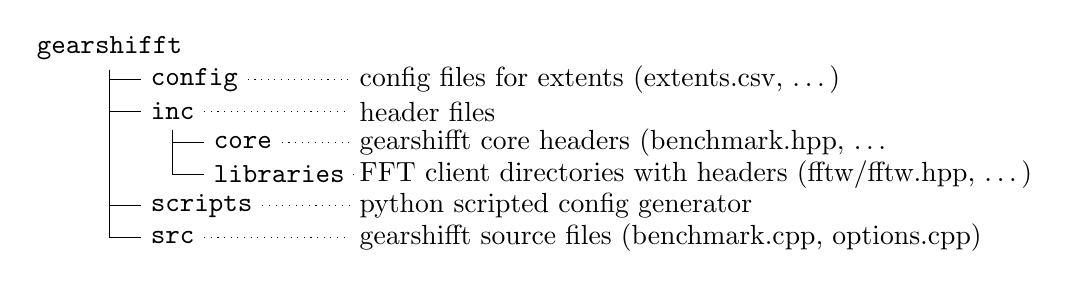
\begin{tikzpicture}
\begin{scope}[grow via three points={one child at (0.4,-0.4) and
  two children at (0.4,-0.4) and (0.4,-0.8)},
  edge from parent path={(\tikzparentnode.south) |- (\tikzchildnode.west)},
  every node/.style={anchor=west,font=\ttfamily}%
]
\node {gearshifft}
    child { node (cfg) {config}}		
    child { node (inc) {inc}
      child { node (core) {core}}
      child { node (lib) {libraries}}
    }
    child [missing] {}				
    child [missing] {}
    child { node (scripts) {scripts}}
    child { node (src) {src}}; 
\end{scope}
\begin{scope}[every node/.style={anchor=west}]
\coordinate (d) at (4.1,0);
\draw[dotted] (cfg) -- (cfg-|d) node { config files for extents (extents.csv, \ldots)};
\draw[dotted] (inc) -- (inc-|d) node { header files};
\draw[dotted] (core) -- (core-|d) node { gearshifft core headers (benchmark.hpp, \ldots};
\draw[dotted] (lib) -- (lib-|d) node { FFT client directories with headers (fftw/fftw.hpp, \ldots)};
\draw[dotted] (scripts) -- (scripts-|d) node { python scripted config generator};
\draw[dotted] (src) -- (src-|d) node { gearshifft source files (benchmark.cpp, options.cpp)}; 
\end{scope}
\end{tikzpicture}
 \caption{gearshifft project structure.}
 \label{fig:projstruct}
\end{figure}



For the command-line arguments Boost is utilized, particularly for benchmark lists and selection. The \gearshifft{} program options are given in \cref{tab:cmdargs}.

\begin{table}[htp]
 \centering
 \caption{gearshifft command-line arguments}
 \label{tab:cmdargs}
  \begin{tabular}{llp{6.4cm}}
\toprule
Flag & [Flag] Argument & Description \\
\midrule
-h&[ -{}-help ]                    &Print help messages \\
-e&[ -{}-extent ] arg              &Specific extent (eg. 1024x1024)\newline[$\ge1$ 
                                  arguments possible] \\
-f&[ -{}-file ] arg                &File with extents (row-wise csv)\newline[$\ge1$ 
                                  arguments possible] \\
-o&[ -{}-output ] arg (=result.csv)&Output csv file, will be overwritten! \\
-v&[ -{}-verbose ]                 &Show statistics after benchmarks finished \\
-d&[ -{}-device ] arg (=gpu)       &Compute device = (gpu|cpu|acc|<ID>). If 
                                  device is not supported by FFT lib, then it
                                  is ignored and default is used. \\
-n&[ -{}-ndevices ] arg (=0)       &Number of devices (0=all), if supported by 
                                  FFT lib (e.g. clfft and fftw with n CPU 
                                  threads). \\
-l&[ -{}-list-devices ]            &List of available compute devices with IDs,
                                  if supported.  \\
-b&[ -{}-list-benchmarks ]         &Show registered benchmarks \\
-r&[ -{}-run-benchmarks ] arg      &Run specific benchmarks (wildcards 
                                  possible, e.g. ClFFT/float/*/Inplace\_Real)\\
\bottomrule
  \end{tabular}
\end{table}



\section{Results}
\label{sec:results}
Based on the experiences made for \cite{preibisch2014efficient, schmid2015real}, this section will discuss results obtained with gearshifft on various hardware in order to showcase the capabilities of \gearshifft{}. We will assume the motivation of a developer seeking to optimize the use of FFTs in the context of the aforementioned publications, i.e. 3D real-to-complex transforms with continguous single-precision input data. If not stated otherwise, this is the transform type assumed for all illustrations hereafter. 

Expeditions into other use cases will be made where appropriate. The curious reader may rest assured that a more comprehensive study is easily possible with \gearshifft{}, however the mere multiplicity of all possible combinations and use cases of FFT render it neither feasible nor practical to discuss 1D or 2D in a comprehensive fashion as well.

For this study, we will concentrate on three modern and current FFT implementations available free of charge: fftw (on x86 CPUs), cufft (on nVidia GPUs) and clfft (on x86 CPUs or nVidia GPUs). We consider this the natural starting point of developers beyond possible domain specific implementations. It should be noted, that this will infer not only a study in terms of hardware performance, but also how well the APIs designed by the authors of fftw, clFFT and cuFFT are documented, understood and used in practise. We consider both hardware and cognitive performance a virtue of almost equal importance.

\subsection{Experimental Environment}
\label{ssec:env}

The results presented in the following sections were collected on three systems:

\begin{itemize}
\item \emph{Taurus HPC cluster}\cite{taurus} running RHEL 7.2
  \begin{itemize}
  \item \emph{K80 node}: 2x Intel(R) Xeon(R) CPU E5-2680 v3 (12 cores) @ 2.50GHz, 64 GB RAM, 4x NVIDIA Tesla K80 (12 GB GDDR5 RAM) GPUs 
  \item \emph{K20X node}: 2x Intel(R) Xeon(R) CPU E5-2450 (8 cores) @ 2.10GHz, 48 GB RAM, 2x NVIDIA Tesla K20x (6 GB GDDR RAM) GPUs 
  \end{itemize}
\item \emph{Hypnos HPC cluster}\cite{hypnos} running Ubuntu 14.04.3:\newline
  2x Intel(R) Xeon(R) CPU E5-2603 v3 @ 1.60GHz, 64 GB RAM (2.67 GB per core), 1x NVIDIA Tesla P100 (16 GB HBM2 RAM) GPUs via PCIe 
\item  \emph{Dell workstation} running CentOS 7.2:\newline 
  2x Intel(R) Xeon(R) CPU E5-2640 v3 @ 2.60GHz, 64 GB RAM, 1x NVIDIA GeForce GTX 1080 (8 GB GDDR5X RAM)
\end{itemize}

As presented above, all used systems operated on a variant of 64-bit Linux and were accessed via an ssh session without running a graphical user interface of any kind. All measurements used the GNU compiler collection (GCC, \cite{stallman2001using}) version 5.3.0 as the underlying compiler if not stated otherwise. 

The FFT implementations evaluated were:

\begin{itemize}
\item fftw \cite{FFTW05}, version 3.3.5
\item cuFFT from CUDA 8.0.44
\item clFFT 2.12.2
\end{itemize}

All used nVidia GPU implementations interfaced with the proprietary driver provided by the vendor. 

In order to generate one data set, a set arrays of arbitrary shapes is provided to a specific FFT API. The configuration files thereof can be accessed via \cite{gearshifft_github}. The shape configurations are separated in groups: \texttt{powerof2} (all dimensions are powers of $2$), \texttt{radix357} (all dimenions are either powers of $3$, $5$ or $7$) and \texttt{oddshape} (all dimenions are powers of $19$ in order to emulated very uncommon signal sizes). These configurations were generated in order to probe the FFT implementations for a wide spectrum of possible applications.  

The FFT calls to benchmark are executed five times each. From this, the arithmetic mean and sample standard deviations are used for figures presented below. As the number of repititions is a configurable parameter of \gearshifft{}, we leave it to the user to produce a more comprehensive data set than used for this publication. We consider five repetitions enough at this point to show and discuss several aspects of performance and usability of \gearshifft{} and the FFT libraries under study.  

%TODO: why maximum size of transforms?

\subsection{Time To Solution}
\label{ssec:tts}

We begin the discussion with the classical use case for developers that might be accustomed to small size transforms. As such, an out-of-place transform with \texttt{powerof2} signal shapes will be assumed.  

\begin{figure}[!tbp]
  \centering
  \def\svgwidth{0.4\columnwidth}
  \subfloat[Fig A.]{\input{figures/k80_cuda8_3d_powerof2_comp.pdf_tex}\label{fig:f1}}
  \hfill
  \def\svgwidth{0.4\columnwidth}
  \subfloat[Fig B.]{\input{figures/k80_cuda8_3d_radix357_comp.pdf_tex}\label{fig:f2}}
  \caption{Some demo figures.}
\end{figure}


% - show measurements
% + K80, GTX 1080, P100
% + Haswell E5

% - analysis starting from 3D
% + inplace versus outplace
% + real vs complex-as-real


\section{Summary}
\label{sec:summary}
% - what can we conclude and recommend by the results?
% - what remains as part of future work?
% - issues?
% - encourage community-driven benchmark?
% - acknowledgements

With this paper, we present \gearshifft{} to the HPC community and other performance enthusiasts as an open-source and free FFT benchmark suite for heterogeneous platforms. \gearshifft{} is a C++14 modular benchmark code that allows to perform forward and backward FFT transforms on various types of input data (both in shape, memory organization, precision and data type). \gearshifft{}'s design offers an extensible architecture to accomodate FFT packages with low overhead. The hallmark of \gearshifft{} is to produce reliable benchmark data that can easily be consumed by external software for visualisation and for easier reproducibility. By these design choices, we hope that \gearshifft{} appeals to both FFT practitioners, FFT library developers and HPC admins or integrators for a wide range of use cases. To show case these capabilities, we presented a first study of common urban myths for using 3 state of the art FFT libraries, fftw, clfft and cufft. We were able to show that the time consumed for the creation of fftw plans can have non-negligible contributions to the time to solution which users of fftw should be aware of. Futhermore, we compared the performance of CPU based implementations Haswell Xeon CPUs to state-of-the-art Pascal generation Nvidia GPUs. We were able to show that for input signal sizes of less than \SI{1}{\mebi\byte}, the CPU implementation is superior whereas for larger input data size the GPU offers better turn-around. The difference between runtimes of power-of-2, {\tt radix357} and power-of-19 shaped input data was demonstrated to be negligible for fftw and non-negligible for cufft transforms used in this study. We were also able to identify runtime differences when using complex versus real arrays and when comparing double versus single precision data types.     

\paragraph{Acknowledgements.} The work of Matthias Werner was funded by Nvidia through the GPU Center of Excellence (GCOE) at the Center for Information Services and High Performance Computing (ZIH), TU Dresden, where the K20Xm and K80 GPU cluster Taurus was used. We would like to thank the Helmholtz-Zentrum Dresden-Rossendorf for providing the infrastructure to host the Nvidia Tesla P100 (provided by Nvidia for the GCOE) in the Hypnos HPC cluster. We would also like to thank the Max Planck Institute of Molecular Cell Biology and Genetics for supporting this publication by providing computing infrastructure and service staff working time.


% allows to break urls at each point
\setcounter{biburllcpenalty}{7000}
\setcounter{biburlucpenalty}{8000}
\printbibliography

\end{document}
